%% Part of Stellarium User Guide 0.15+
%% History:
%% 2016-04-17 New chapter.
%% !!!!!!!!!! Please ask GZ before editing this file. !!!!!!!!!!!!!!!


% \chapter{Cultural Astronomy}
% \label{ch:CulturalAstronomy}
% \chapterauthor*{Georg Zotti}
% 
% \noindent \indexterm{Cultural astronomy} describes how astronomy, ritual or
% systematic observation of celestial objects influences the daily life
% of past and present cultures. It encloses astronomical elements of
% calendar making, worship, navigation, celestial mythology, starlore
% and other things not mentioned here.
% 
% Stellarium is a wonderful tool to visualize the sky, celestial
% objects, mythological figures, and the landscape, together describes
% as the \indexterm{skyscape}. The Scenery3D plugin has been described
% in chapter~\ref{ch:Scenery3D}, but apart from this there are more
% extensions which are of interest.
% 
\newpage
\section{ArchaeoLines Plugin}
\label{sec:plugin:ArchaeoLines}

\begin{figure}[ht]
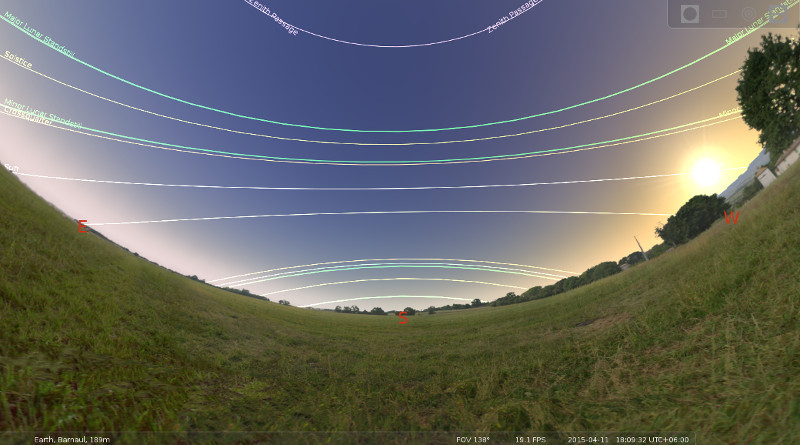
\includegraphics[width=\textwidth]{ArchaeoLines.jpg}
\caption{Declination Lines provided by the ArchaeoLines plugin}
\label{fig:plugin:ArchaeoLines}
\end{figure}


\subsection{Introduction}
\label{sec:plugin:ArchaeoLines:Introduction}

In the archaeoastronomical literature, several astronomically derived
orientation schemes are prevalent. Often prehistorical and historical
buildings are described as having been built with a main axis pointing
to a sunrise on summer or winter solstice. There can hardly be a
better tool than Scenery3D (see chapter~\ref{ch:scenery3d}) to
investigate a 3D model of such a building, and this plugin has been
introduced in version 0.13.3 as a further tool in the
archaeoastronomer's toolbox.

When activated (see section~\ref{sec:Plugins:EnablingPlugins}), there
is a tool bar button \guibutton{0.6}{bt_archaeolines} (in the
shape of a \emph{trilithon} with the sun shining through it). Press
this, or \key{\ctrl+U}, to display the currently selected set of
characteristical diurnal arcs.

\subsection{Characteristic Declinations}
\label{sec:plugin:ArchaeoLines:Declinations}


The ArchaeoLines plugin displays any combination of declination arcs most
relevant to archaeo- or ethnoastronomical studies. Of course, principles
used in this context are derived from natural observations, and many of
these declinations are still important in everyday astronomy.

\begin{itemize}
\item Declinations of equinoxes (i.e., the equator) and the solstices
\item Declinations of the crossquarter days (days right between solstices and equinoxes)
\item Declinations of the Major Lunar Standstills
\item Declinations of the Minor Lunar Standstills
\item Declination of the Zenith passage
\item Declination of the Nadir passage
\item Declination of the currently selected object
\item Current declination of the sun
\item Current declination of the moon
\item Current declination of a naked-eye planet
\end{itemize}

\noindent For the lunar events, there are two lines each drawn, for
maximum and minimum distance of the moon.  The lunar extreme
declinations are computed taking horizon parallax effects into
account. Fore technical reasons however, the derived declinations are
then used to draw \emph{small circles} of constant declinations on the
sphere, without taking the change of lunar horizontal parallax into
account.  Note that therefore the observed declination of the moon at
the major standstill can exceed the indicated limits if it is high in
the sky.

It may be very instructive to let the time run quite fast and observe
the declination line of ``current moon'' swinging between its north
and south limits each month.  These limits grow and shrink between the
Major and Minor Standstills in the course of 18.6 years.

The sun likewise swings between the solstices. Over centuries, the
solstice declinations very slightly move as well due to the slightly
changing obliquity of the ecliptic.


\subsection{Configuration Options}
\label{sec:plugin:ArchaeoLines:configuration}

The configuration dialog allows the selection of the lines which are
of interest to you. 
%
%For example, in Mesoamerica the Lunar standstills
%seem not to be relevant, while zenith and nadir passages seem to have
%been important. Also Venus or other planets may appear useful.
%
In addition, you can select the color of the lines by clicking on the
color swatches.\footnote{Unfortunately, on Windows, the color dialog hides
behind the Stellarium window when in fullscreen mode. So, before
editing line colors, please leave fullscreen mode!}

\subsection*{Section [ArchaeoLines] in config.ini file}

Apart from changing settings using the plugin configuration dialog,
you can also edit \file{config.ini} file by yourself for changes of the
settings for the ArchaeoLines plugin -- just make it carefully!

\begin{longtabu} {l|l|l}\toprule
\emph{ID}                   &\emph{Type} & \emph{Default}  \\\midrule
enable\_at\_startup         &bool        & false           \\\midrule
color\_equinox              &float R,G,B & 1.00,1.00,0.5   \\\midrule
color\_solstices            &float R,G,B & 1.00,1.00,0.25  \\\midrule
color\_crossquarters        &float R,G,B & 1.00,0.75,0.25  \\\midrule
color\_major\_standstill    &float R,G,B & 0.25,1.00,0.25  \\\midrule
color\_minor\_standstill    &float R,G,B & 0.20,0.75,0.20  \\\midrule
color\_zenith\_passage      &float R,G,B & 1.00,0.75,0.75  \\\midrule
color\_nadir\_passage       &float R,G,B & 1.00,0.75,0.75  \\\midrule
color\_selected\_object     &float R,G,B & 1.00,1.00,1.00  \\\midrule
color\_current\_sun         &float R,G,B & 1.00,1.00,0.75  \\\midrule
color\_current\_moon        &float R,G,B & 0.50,1.00,0.50  \\\midrule
color\_current\_planet      &float R,G,B & 0.25,0.80,1.00  \\\midrule
show\_equinox               &bool        & true  \\\midrule
show\_solstices             &bool        & true  \\\midrule
show\_crossquarters         &bool        & true  \\\midrule
show\_major\_standstills    &bool        & true  \\\midrule
show\_minor\_standstills    &bool        & true  \\\midrule
show\_zenith\_passage       &bool        & true  \\\midrule
show\_nadir\_passage        &bool        & true  \\\midrule
show\_selected\_object      &bool        & true  \\\midrule
show\_current\_sun          &bool        & true  \\\midrule
show\_current\_moon         &bool        & true  \\\midrule
show\_current\_planet       &bool        & true  \\\bottomrule
\end{longtabu}


% \section{Adding Sky Cultures}
% \label{sec:SkyCultures}
% 
% Stellarium comes with a nice set of skycultures. For ethnographers or
% historians of science it may be a worthwile consideration to
% illustrate the sky culture of the people they are studying. It is not
% very hard to do so, but depending on your data, may require some
% skills in image processing.
% 
% TO BE CONTINUED.
% 

%%% Local Variables: 
%%% mode: latex
%%% TeX-master: "guide"
%%% End: 

